\section{Experiment}
\iffalse
https://github.com/HAIRLAB/Pre_Surv_COVID_19/

The choice of the cell is usually guided by the task at hand [J. Chung, C. Gulcehre, K. Cho, and Y. Bengio. Empirical evaluation of gated recurrent neural networks on sequence modeling.].
In all experiments we use an AE with 3 hidden layers, { D x , 30, D z , 30, D x } ; the number of neurons in the intermediate layers (30) has been set after preliminary experiments and is not a critical hyperparameter (comparable results were obtained using 20 or 40 neurons).
% In each experiment, we train the models for 5000 epochs with mini-batches containing 32 MTS using the Adam optimizer [kingma2014adam, D. Kingma and J. Ba. Adam: A method for stochastic optimization.] with an initial learning rate of 0.001.
% Data are in random order
% We consider the problem of classifying patients with and without surgical site infections from their blood samples.
% However, an important question for any autoencoder-style model is what prevents it from learning an identity mapping and effectively copying the input to the output. In that case all the information about the input would still be present but the representation will be no better than the input. There are two factors that control this behaviour. First, the fact that there are only a fixed number of hidden units makes it unlikely that the model can learn trivial mappings for arbitrary length input sequences.
% For this purpose, machine learning tools selected three biomarkers that predict the mortality of individual patients more than 10 days in advance with more than 90\% accuracy:

The problem was formulated as a classification task, where the inputs included basic information, symptoms, blood samples and the results of laboratory tests, including liver function, kidney function, coagulation function, electrolytes and inflammatory factors, taken from originally general, severe and critical patients (Table 1), as well as their associated outcomes corresponding to either survival or death at the end of the examination period. 
Medical records were collected by using standard case report forms that included epidemiological, demographic, clinical, laboratory and mortality outcome information (Table 2 and Supplementary Data 1).
The clinical outcomes were followed up to 24 February 2020.
% The medical information of all patients collected between 10 January and 18 February 2020 were used for model development.
Of the 375 cases included in the subsequent analysis, 201 recovered from COVID-19 and were discharged from the hospital, while the remaining 174 died> deceased.
% The performance models were evaluated by assessing the classification accuracy (ratio of true predictions over all predictions), the precision, sensitivity/recall and F1 scores (defined below): Definition of metrics with TP FP TN FN.

Selecting how deeper the model should be is another aspect of hyperparameter optimisation which can generally go from a single layer to three to four-layer deep model architecture where a three-layer architecture is used mostly in complex learning tasks. 

Because of the rapid spread of the virus, there has been a sharp increase in the demand for medical resources required to support infected people. Despite the desperate efforts to contain the disease and slow down its spread, many countries have been suffering from the shortage of hospital beds and critical care equipment for the timely treatment of ill patients[Ranney, M. L., Griffeth, V. & Jha, A. K. Critical supply shortages—The need for ventilators and personal protective equipment during the Covid-19 pandemic.,Gondi, S. et al. Personal protective equipment needs in the USA during the COVID-19 pandemic., Smereka, J. & Szarpak, L. The use of personal protective equipment in the COVID-19 pandemic era.]. Therefore, in addition to efficient diagnosis and treatment, accurate prognosis prediction is necessary to reduce the strain on healthcare systems and provide the best possible care for patients. When allocating limited medical resources, prediction models that estimate the risk of a poor outcome in an infected individual based on pre-diagnosis information could help to effectively triage patients.

In order to study the important blood biomarkers for predicting disease mortality, a retrospective study was conducted on 375 COVID- 19 positive patients admitted to Tongji Hospital (China) from January 10 to February 18, 2020. Demographic and clinical characteristics, and patient outcomes were investigated using machine learning tools to identify key biomarkers to predict the mortality of individual patient. A nomogram was developed for predicting the mortality risk among COVID-19 patients.

Yan et al. [21] reported a machine learning approach to select three biomarkers (lactic dehydrogenase (LDH), lymphocyte and high-sensitivity C-reactive protein (hs-CRP)) and using them to predict individual patients mortality, 10 days ahead with more than 90 percent accuracy. 
Blood samples collected between 10 January and 18 February, 2020 from 375 patients in Wuhan, China were retrospectively analyzed to identify reliable and relevant markers of mortality risk. Medical records were collected using standard case report forms, which included information on epidemiological, demographic, clinical, laboratory and mortality outcomes. Yan et al. [21] has published the dataset along with the article and the original study was approved by the Tongji Hospital Ethics Committee. Patients’ exclusion criteria for the study were: Age (<18 years), pregnant, breast- feeding and missing data (>20\%). Out of 375 patients, 187 (49.9\%) had fever while cough, fatigue, dyspnea, chest distress and muscular soreness were present in 52 (13.9\%), 14 (3.7\%), 8 (2.1\%), 7 (1.9\%) and 2 (0.5\%) patients respectively.
Of the 375 patients, 174 (46.4\) died, while 201 (53.6\%) patients recovered from COVID-19 and were discharged from hospital. Figure 1 summarizes the outcome of patients based on their initial conditions: general (197), severe (27) and critical (151). The minimal, maximal and median follow-up times (from hospital admission to death or discharge) for all 375 patients are 0 days, 35 days and 12 days, respectively.
Table 1 summarizes the demographic characteristics, clinical characteristics, and clinical outcomes of the subjects in the death and survival groups. There were 142 (37.9\%) patients, who were Wuhan residents, 2 (0.5\%) had contact with confirmed or suspected patients, 24 (6.4\%) were from familial cluster, 7 (1.9\%) were health workers, 2 (0.5\%) had contact with Huanan Seafood Market and 198 (52.5\%) had no contact history.

The main problem of neural networks, and therefore also of LSTMs, is the fact that is not always easy to understand how the network can identify the relationship between the input data and the target class.
\fi
%%%%%%%%%%%%%%%%%%%%%%%%%%%%%%%%%%%%%%%%%%%%%%%%%%%%%%%%%%%%%%%%%%%%%%%%%%%%%%%%%%%
%% Precision and Recall on what? on survival and death both?
% [We design experiments to accomplish the following objectives:]
% Experiment section is organized as follows:
% 1. Prediction Performance on Classification on mortality.
% 2. blah.
% Convergency graph where all k-th runs are in a single figure.

\subsection{Dataset}
% Normalized, Min-max scaling. Time point to floating numbers, seconds after admission.
We obtain the blood sample records, basic demographic information, and associated mortality outcomes of 375 patients collected throughout their stay in hospital from Tongji Hospital between 10th January and 24th February 2020 following the previous research~\cite{yan2020interpretable}. We discard 17 samples whose no time stamp is recorded. Among the remaining 358 samples, 192 patients survived (labeled by 1) and 166 patients died (labeled by 0). The order of samples is randomly shuffled to prevent the bias from the order. The missing entries are initialized as -1. Each feature of dataset is normalized by min-max scaling to the range [0, 1]. 

\subsection{Hyperparameters}
We find the best hyperparameters of our model by the grid search; LSTM units in \{64, 100, 128\}, $\gamma_1$ and $\gamma_2$ in $\{1e-1,\ 1e-2,\ 1e-3\}$, and learning rate of optimizer in $\{1e-2,\ 1e-3,\ 1e-4,\ 1e-5\}$. We construct the decoder and predictor with 3 hidden layers, and the number of hidden layers and units of each layer does not impact the performance significantly. We use hyperbolic tangent activation function for all layers, except logistic sigmoid function at the output layer of predictor, and leaky Rectified Linear Unit (leaky ReLU, alpha = 0.1) at the input layer of decoder. We note that the leaky ReLU have been largely improved the reconstruction performance of decoder, as we presume that time stamp is the most important input for the decoder and this can be emphasized more with leaky ReLU activation function in a range $(- \infty, \infty)$, than the other activation functions in a smaller range. The mini batch size is set to 1. We do not use any regularization or dropout technique, as they are found to degrade the performance. We minimize the loss function in Eq.~\eqref{eq: objective} with Adam optimizer~\cite{kingma2014adam}.
% For prediction error, we have tried binary cross entropy and mean squared error, and mean squared error works better. Best Hyper-parameters are searched by following set of grid. Because RE\_DATE is important feature in decoder input, thus should be emphasized, we use leaky ReLU activation function at the input layer of decoder. And the prediction accuracy is improved with leaky ReLU at the input layer than tanh, while tanh works better in other layers.

\subsection{Mortality Classification Task}
%% Simple LSTM is ablation study.
To evaluate the prediction performance of the proposed model, we consider the classification problem to predict the mortality of COVID-19 patients in advance more than 10 days. The output of predictors are rounded up to the binary. We compare the accuracy, precision, recall, and $\text{F}_1$-score of our model (Semi-supervised AutoEncoder, SAE) to those metrics of the other baseline supervised learning models. The pure LSTM model is introduced for the ablation study, and it consists of LSTM encoder and MLP predictor same as our model, but the decoder is removed. We conduct the k-fold cross validation by splitting the dataset samples into k sub-groups, and calculate the average and standard deviation of the four metrics over the k sub-groups. The baseline supervised learning models are trained on the training set, while our semi-supervised learning model is trained on training and test set both. The blood sample records at all the time points are given to  the time series models, LSTM and SAE, while the blood sample record only at the last time point is given to the other baseline models. The demographic information, age, gender, admission time, discharge time, are provided as the static record to all prediction models.
% SAE, LSTM, MLP, LASSO, RR, SVM denote the Semi-supervised LSTM Auto Encoder (our model), Long Short Term Memory, Multi Layer Perceptron, Least Absolute Shrinkage and Selection Operator, Ridge Regression, Support Vector Machine, respectively.
% From the 75 dynamic features from blood samples, and 4 static features from patient's demographic, we predict the patient's mortality in 10 days.
% **************** Forgot to mention the definition of baseline models.
\begin{table*}[h]\label{tab: experimetal results}
    % \footnotesize
    %\scriptsize
    \small
    \setlength{\tabcolsep}{4pt} %% change column-wise separation.
    \centering
    \caption{The prediction results of SAE and the baseline models from k-fold cross validation. The best prediction is denoted as bold font.}\label{tab: prediction RMSE}
    \begin{tabular}{|c|c|c|c|c|c|} %% 6 columns table
    \hline
    {\bfseries Test Set Size} & {\bfseries Model} & \multicolumn{1}{c}{{\bfseries Accuracy}} & \multicolumn{1}{c}{{\bfseries Precision}} & \multicolumn{1}{c}{{\bfseries Recall}} & {\bfseries $\text{F}_1$-score}\\ %% Headers
    \Xhline{1pt}
    \multirow{6}{*}{20\%} %% 6 rows group.
    & SAE & \multicolumn{1}{c}{{\bfseries 94.14$\pm$2.31}} & \multicolumn{1}{c}{\bfseries{93.35$\pm$2.45}} & \multicolumn{1}{c}{{\bfseries 93.15$\pm$2.84}} & {\bfseries 93.48$\pm$1.21}\\
    & LSTM & \multicolumn{1}{c}{92.56$\pm$3.24} & \multicolumn{1}{c}{91.11$\pm$1.45} & \multicolumn{1}{c}{92.45$\pm$8.12} & 91.43$\pm$5.40\\
    & MLP & \multicolumn{1}{c}{80.63$\pm$11.52} & \multicolumn{1}{c}{76.58$\pm$10.94} & \multicolumn{1}{c}{83.80$\pm$11.97} & 80.02$\pm$11.14\\
    & RF & \multicolumn{1}{c}{83.25$\pm$11.89} & \multicolumn{1}{c}{78.03$\pm$11.15} & \multicolumn{1}{c}{88.77$\pm$12.68} & 83.05$\pm$11.86\\
    & RR & \multicolumn{1}{c}{79.32$\pm$11.33} & \multicolumn{1}{c}{76.76$\pm$10.97} & \multicolumn{1}{c}{79.54$\pm$11.36} & 78.12$\pm$11.16\\
    & SVM & \multicolumn{1}{c}{79.32$\pm$11.33} & \multicolumn{1}{c}{77.55$\pm$11.08} & \multicolumn{1}{c}{78.12$\pm$11.16} & 77.83$\pm$11.11\\
    \Xhline{1pt}
    \multirow{6}{*}{25\%} %% 6 rows group.
    & SAE & \multicolumn{1}{c}{{\bfseries 92.47$\pm$3.43}} & \multicolumn{1}{c}{{\bfseries 91.84$\pm$8.41}} & \multicolumn{1}{c}{{\bfseries 91.97$\pm$2.34}} & {\bfseries 91.63$\pm$3.94}\\
    & LSTM & \multicolumn{1}{c}{91.91$\pm$3.69} & \multicolumn{1}{c}{91.38$\pm$8.94} & \multicolumn{1}{c}{91.62$\pm$1.89} & 91.17$\pm$3.98\\
    & MLP & \multicolumn{1}{c}{81.90$\pm$11.70} & \multicolumn{1}{c}{79.25$\pm$11.32} & \multicolumn{1}{c}{82.92$\pm$11.85} & 81.05$\pm$11.58\\
    & RF & \multicolumn{1}{c}{83.30$\pm$11.9} & \multicolumn{1}{c}{78.94$\pm$11.28} & \multicolumn{1}{c}{87.45$\pm$12.49} & 82.98$\pm$11.85\\
    & RR & \multicolumn{1}{c}{80.50$\pm$11.50} & \multicolumn{1}{c}{81.13$\pm$11.16} & \multicolumn{1}{c}{76.14$\pm$10.88} & 78.56$\pm$11.22\\
    & SVM & \multicolumn{1}{c}{80.50$\pm$8.12} & \multicolumn{1}{c}{80.11$\pm$11.45} & \multicolumn{1}{c}{77.65$\pm$11.09} & 78.86$\pm$11.27\\
    \Xhline{1pt}
    \multirow{6}{*}{75\%} %% 6 rows group.
    & SAE & \multicolumn{1}{c}{{\bfseries 89.48$\pm$1.59}} & \multicolumn{1}{c}{{\bfseries 88.59$\pm$2.27}} & \multicolumn{1}{c}{88.72$\pm$6.09} & {\bfseries 88.46$\pm$2.1}\\
    & LSTM & \multicolumn{1}{c}{87.91$\pm$1.07} & \multicolumn{1}{c}{87.41$\pm$3.22} & \multicolumn{1}{c}{86.07$\pm$4.59} & 86.57$\pm$1.4\\
    & MLP & \multicolumn{1}{c}{80.09$\pm$11.44} & \multicolumn{1}{c}{74.94$\pm$10.71} & \multicolumn{1}{c}{86.86$\pm$12.41} & 80.46$\pm$11.50\\
    & RF & \multicolumn{1}{c}{88.52$\pm$12.65} & \multicolumn{1}{c}{85.49$\pm$12.21} & \multicolumn{1}{c}{{\bfseries 91.32$\pm$13.0}} & 88.31$\pm$12.62\\
    & RR & \multicolumn{1}{c}{79.03$\pm$11.29} & \multicolumn{1}{c}{75.54$\pm$10.79} & \multicolumn{1}{c}{82.41$\pm$11.77} & 78.82$\pm$11.26\\
    & SVM & \multicolumn{1}{c}{77.98$\pm$11.11} & \multicolumn{1}{c}{75.06$\pm$10.7} & \multicolumn{1}{c}{80.18$\pm$11.45} & 77.54$\pm$11.08\\
    \Xhline{1pt}
    \multirow{6}{*}{80\%} %% 6 rows group.
    & SAE & \multicolumn{1}{c}{{\bfseries 88.06$\pm$1.07}} & \multicolumn{1}{c}{{\bfseries 86.98$\pm$1.82}} & \multicolumn{1}{c}{{\bfseries 87.03$\pm$3.29}} & {\bfseries 86.95$\pm$1.44}\\
    & LSTM & \multicolumn{1}{c}{84.07$\pm$5.55} & \multicolumn{1}{c}{86.55$\pm$2.91} & \multicolumn{1}{c}{77.60$\pm$16.00} & 80.66$\pm$9.94\\
    & MLP & \multicolumn{1}{c}{79.46$\pm$11.35} & \multicolumn{1}{c}{72.80$\pm$10.40} & \multicolumn{1}{c}{82.19$\pm$11.17} & 77.21$\pm$11.03\\
    & RF & \multicolumn{1}{c}{51.15$\pm$4.09} & \multicolumn{1}{c}{64.18$\pm$14.00} & \multicolumn{1}{c}{30.00$\pm$25.83} & 59.81$\pm$16.37\\
    & RR & \multicolumn{1}{c}{78.14$\pm$11.16} & \multicolumn{1}{c}{70.78$\pm$10.11} & \multicolumn{1}{c}{82.19$\pm$11.17} & 76.06$\pm$10.87\\
    & SVM & \multicolumn{1}{c}{74.16$\pm$10.79} & \multicolumn{1}{c}{66.22$\pm$9.46} & \multicolumn{1}{c}{79.03$\pm$11.3} & 72.06$\pm$10.29\\
    \cline{1-6}
    \end{tabular}
\end{table*}

The experimental results in Table~\ref{tab: experimetal results} show that our model outperforms the other baseline models for all the different size of test sets. The performance improvement's margins of our model respect to the baseline models are larger when the smaller size of training set (which means the larger size of test set) is given. We suppose this is because our model is able to learn from the unlabeled samples, while the other supervised learning models are able to learn from only the labeled samples. The unlabeled samples are also useful resources for our model to improve the enrichment capability, which can help the prediction from the enriched representation.
\subsection{Biomarker Identification}
We identifies which biomarkers of blood samples are the risk factors for the mortality of COVID-19 patients. Despite the high performance of artificial neural networks, the outputs of artificial neural networks are notoriously difficult to be interpreted. To identify which biomarkers largely affect to the predictions, we add the perturbations to the input time series and observe the prediction changes. We try to perturb each feature of time series in the range of the distribution of the feature.

For $m$-th feature ($1 \leq m \leq D_l$) and $i$-th patient, we sample the column vector of perturbation $\mathbf{p}_{i,m} \in \Re^{n_i}$ from the normal distribution $\mathcal{N}(0, \sigma_m^2)$ with zero mean and the same standard deviation as the distribution of $m$-th feature across all the time and patients, as follows:
\begin{equation}
\begin{aligned}
    &N = \sum_{i=1}^n \sum_{j=1}^{n_i} m^j_i,\ \mu_m = \frac{1}{N}\sum_{i=1}^n \sum_{j=1}^{n_i} m_i^j * x_i^j,\\
    &\sigma_m^2 = \frac{1}{N}\sum_{i=1}^n \sum_{j=1}^{n_i} m_i^j(x_i^j - \mu_m)^2.
\end{aligned}
\end{equation}
Then the time series whose $m$-th feature is perturbed and it's prediction change is:
\begin{equation}
\begin{aligned}
    &\mathbf{X}_i' = [\mathbf{x}_{i, 1}, \mathbf{x}_{i, 2}, \cdots, \mathbf{x}_{i, m} + \mathbf{p}_{i, m}, \cdots, \mathbf{x}_{i, D_l}],\\
    &\Delta\tilde{\mathbf{y}}_i = \| \phi_P(\phi_E(\mathbf{X}_i, \mathbf{M}_i, \mathbf{t}_i; \mathbf{\theta}_E), \mathbf{x}_i^s; \mathbf{\theta}_P) - \phi_P(\phi_E(\mathbf{X}_i', \mathbf{M}_i, \mathbf{t}_i; \mathbf{\theta}_E), \mathbf{x}_i^s; \mathbf{\theta}_P) \|,
\end{aligned}
\end{equation}
where $\mathbf{x}_{i, m} \in \Re^{n_i}$ is the column vector of feature observations of $i$-th patient across all the time points. Then the relative importance of $m$-th feature is the average of prediction changes across all the patients: $\frac{1}{n}\sum_{i=1}^n\Delta\tilde{\mathbf{y}}_i$. Finally, we plot top 15 most important features in Fig.~\ref{fig: identified-features}.

\begin{figure}[h]
    \raggedright
    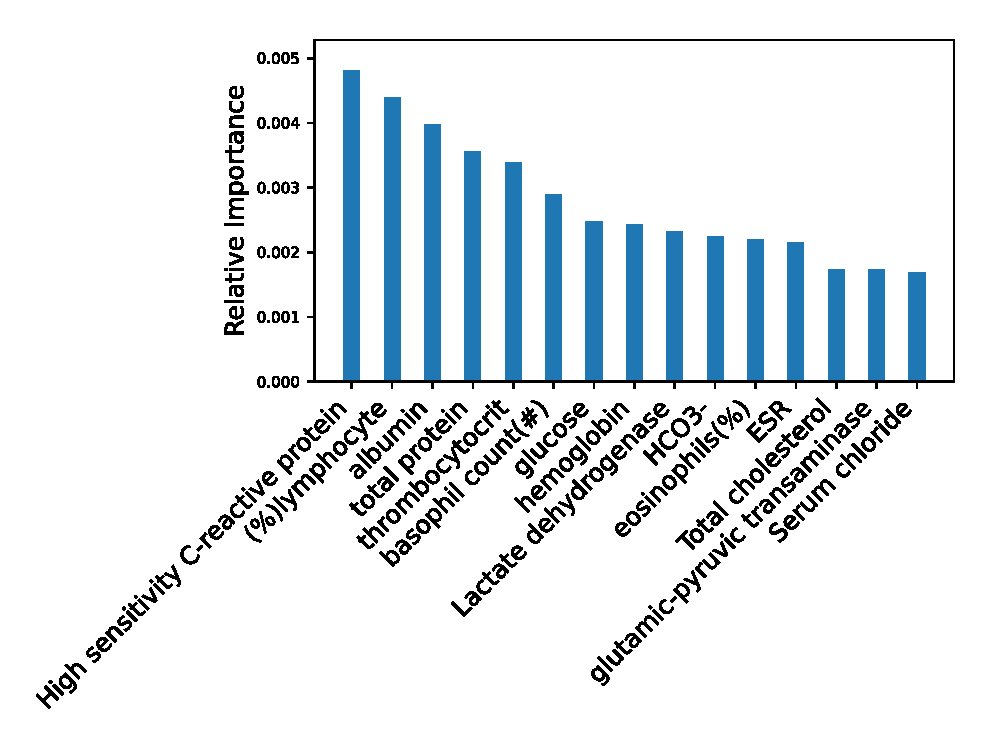
\includegraphics[width=0.85\textwidth]{figures/identified-features.eps}
    \caption{Top 15 important biomarkers identified by the proposed model.} \label{fig: identified-features}
\end{figure}
Some of the identified biomarkers are consistent with the previous medical findings. For example, lactic dehydrogenase (LDH), lymphocyte and high-sensitivity C-reactive protein (hs-CRP) are the top 3 biomarkers relevant with the mortality of COVID-19 patients, identified by the XGBoost model \cite{yan2020interpretable} and previous medical researches~\cite{kishaba2014staging,ridker2008rosuvastatin,wang2020clinical}. % 11, 12, 16 cited.
To be specific, the increase of LDH indicates tissue or cell destruction and this is the strong sign of tissue or cell damage~\cite{yan2020interpretable}. The activity of idiopathic pulmonary fibrosis can be detected by Serum LDH~\cite{kishaba2014staging}. The hs-CRP is the risk factor for the continuous inflammation~\cite{bajwa2009plasma} and poor prognosis in acute respiratory distress syndrome~\cite{kishaba2014staging,sharma2016aetiology}. The lymphocyte is the common risk factor of COVID-19 patients~\cite{chan2020familial}, and lymphocyte has relation with the decrease in CD4 and CD8 T cells~\cite{liu2020longitudinal}.
Albumin have been found to be independently associated with mortality, at the Cox regression analysis~\cite{violi2020albumin}. The basophil count is known to be the risk factor of mortality and organ injury in COVID-19 patients~\cite{li2020immune}. The identified biomarkers are supported by the previous studies, and add the value on our semi-supervised prediction model and perturbation based analysis.
% Pure LSTM

% The experimental result in \ref{tab: experimetal results} shows 
% It is validation accuracy on test set, not a training set. Output layer of predictor uses sigmoid activation function, and round up the output to generate binary class.

% \subsection{Reconstruction}
% Loss value changes by whether label is given or not, but loss converges stably. : convergency graph.

%% Low standard devation and large test set -> The prediction is stable and robust.

%%% COVID-19 risk factors previous studies.
%% Neutrophil-to-lymphocyte : Neutrophil-to-lymphocyte ratio as an independent risk factor for mortality in hospitalized patients with COVID-19, Yuwei Liu.